\documentclass[prb,twocolumn]{revtex4-2}
\usepackage{graphicx}
\usepackage{amsmath}
\usepackage{amssymb}
\usepackage{epstopdf}

\begin{document}
\title{Assignment 3}

\author{James Lawton}
\affiliation {
Physics Department, Virginia Tech, Blacksburg, Virginia 24061, USA\\
}


\begin{abstract}
Absract: A few sentences summarizing the topics of each problem.  The document should be in APS PRB format.  
\end{abstract}

\maketitle

\section{Problem 1}

\noindent
Here we look to find a root for the equation $f(x)=e^{x^2}ln(x^2)-x$, utilizing an implimentation of the secant method. We look at how the delta ($\delta$) affects how close the program gets to the true root value.

The secant method is similar to Newton's method, only it doesn't require knowing the derivative of the function: It takes two starting points instead of one and draws a secant line from them which should (hopefully) intersect with the x-axis. The value is taken from that intersection and plugged back into the equation. The first guess point is replaced with the second, and the second is replaced with the point that was just obtained. This process is repeated until a guess is within a distance of $\delta$ to the previous guess.

The simulation was run with $\delta$ ranging from $10^{-100}$ to $10^{-10}$, anything larger yielded a single value. The results plotted the root value obtained over $\delta$:

\begin{figure}[h!]
\centerline{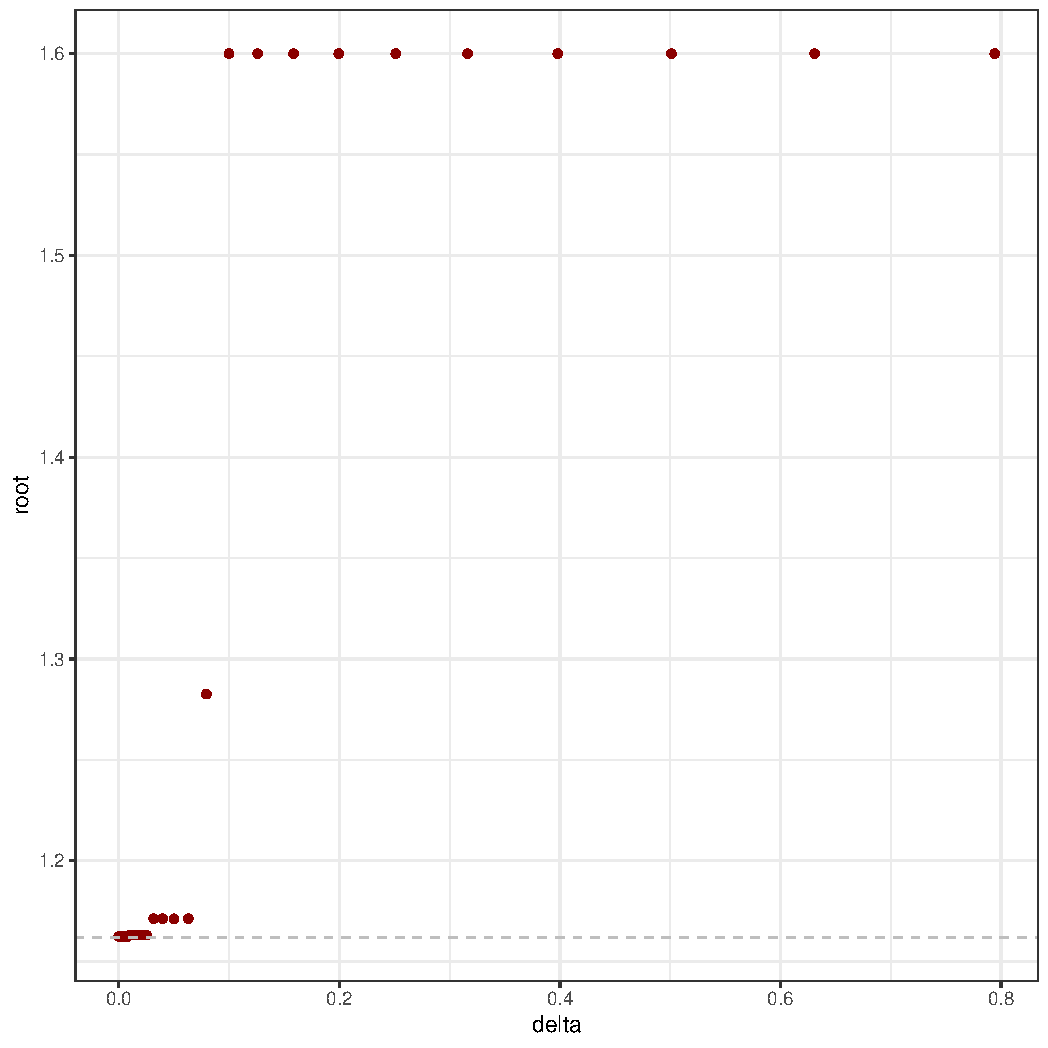
\includegraphics [width=3 in] {secant}} \caption{Secant Method} \label{secant}
\end{figure}

Here it's clear that smaller values of delta yield results that are closer to the true root, represented with a gray dotted line. We can also see that there are clear "steps" as we get closer and closer to the root, starting at $1.6$, representing each step the secant method takes to get to the root.

\section{Problem 2}

Here we look to use an implimentation of Newton's method to solve a system of equations:

\begin{eqnarray}
f_1(x_1,x_2)=e^{x_1^2}ln(x_2)-x_1 \\
f_2(x_1,x_2)=e^{x_2}ln(x_1)-x_2^2
\label{namefornewequation}
\end{eqnarray}
We look at how the delta ($\delta$) affects how close the program gets to the true root value.

Newton's method has a few differences when using it on multidimensional systems of equations.

\begin{eqnarray}
x_{n+1}=x_n+\frac{f(x_n)}{f(x_n)} \\
\bold{f(x+\Delta x)}=\bold{f(x)}+\bold{J(x)\Delta x} \\
-\bold{f(x)}\approx\bold{J(x)\Delta x}
\label{namefornewequation}
\end{eqnarray}

LU decomposition is used to solve equation 5 for $\bold{\Delta x}$.


The simulation was run with $\delta$ ranging from $10^{-10}$ to $1$, The results plotted the root value's y component over it's x component with the color gradient representing $\delta$:

\begin{figure}[h!]
\centerline{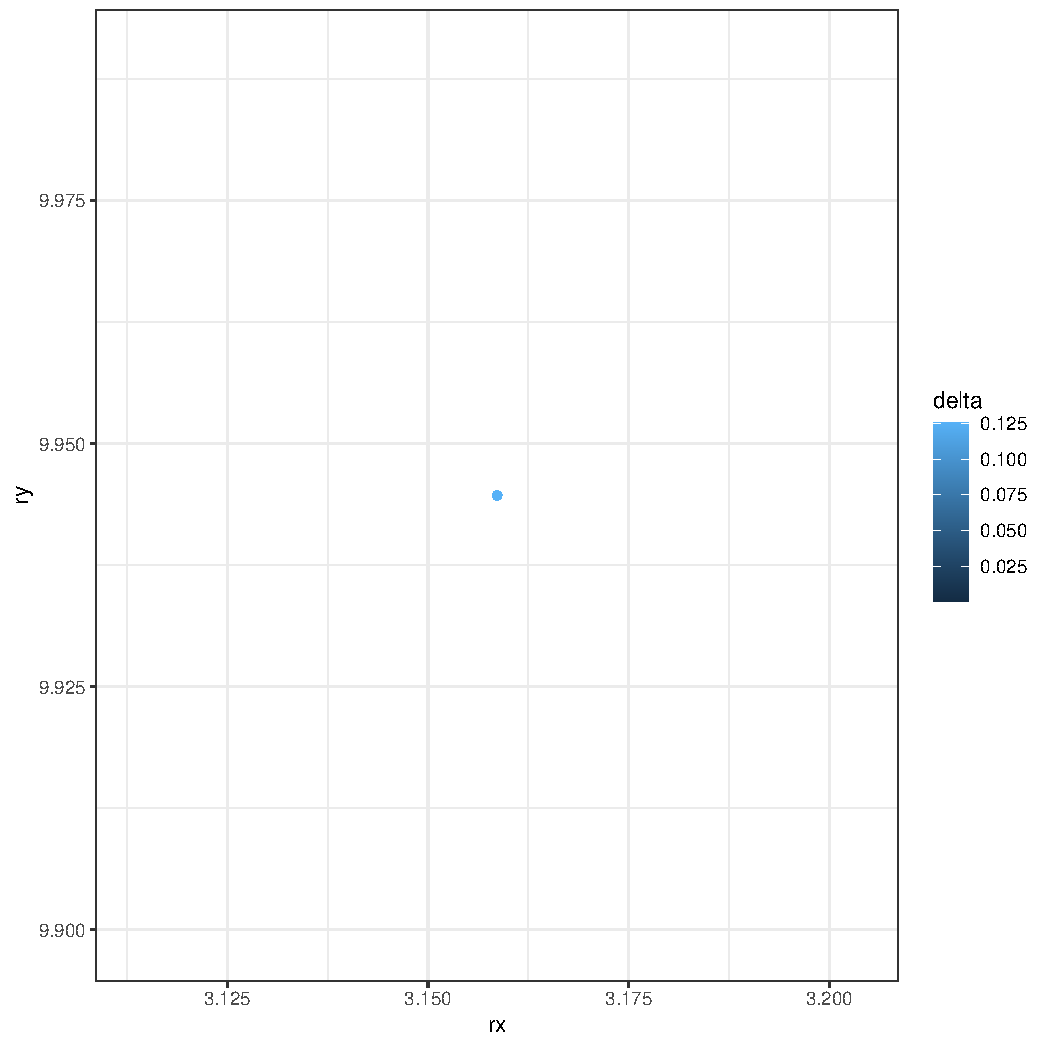
\includegraphics [width=3 in] {newton}} \caption{Multidimensional Newton Method} \label{newton}
\end{figure}

Something clearly went wrong in the code here as the root values stay at one point. Ideally we would be able to see the path the algorithm takes to obtain the root with a gradient color as it approaches.

\section{Problem 3a}

Here we look to calculate the value of the following integral using Simpson's Method.

\begin{eqnarray}
S = \int_{-\infty}^\infty e^{x^2}dx
\label{namefornewequation}
\end{eqnarray}

This simulation was run with an $n$ value ranging from 1 to 20 which is when there becomes no more visible variation. The $S$ value is then plotted over $n$. 

\begin{figure}[h!]
\centerline{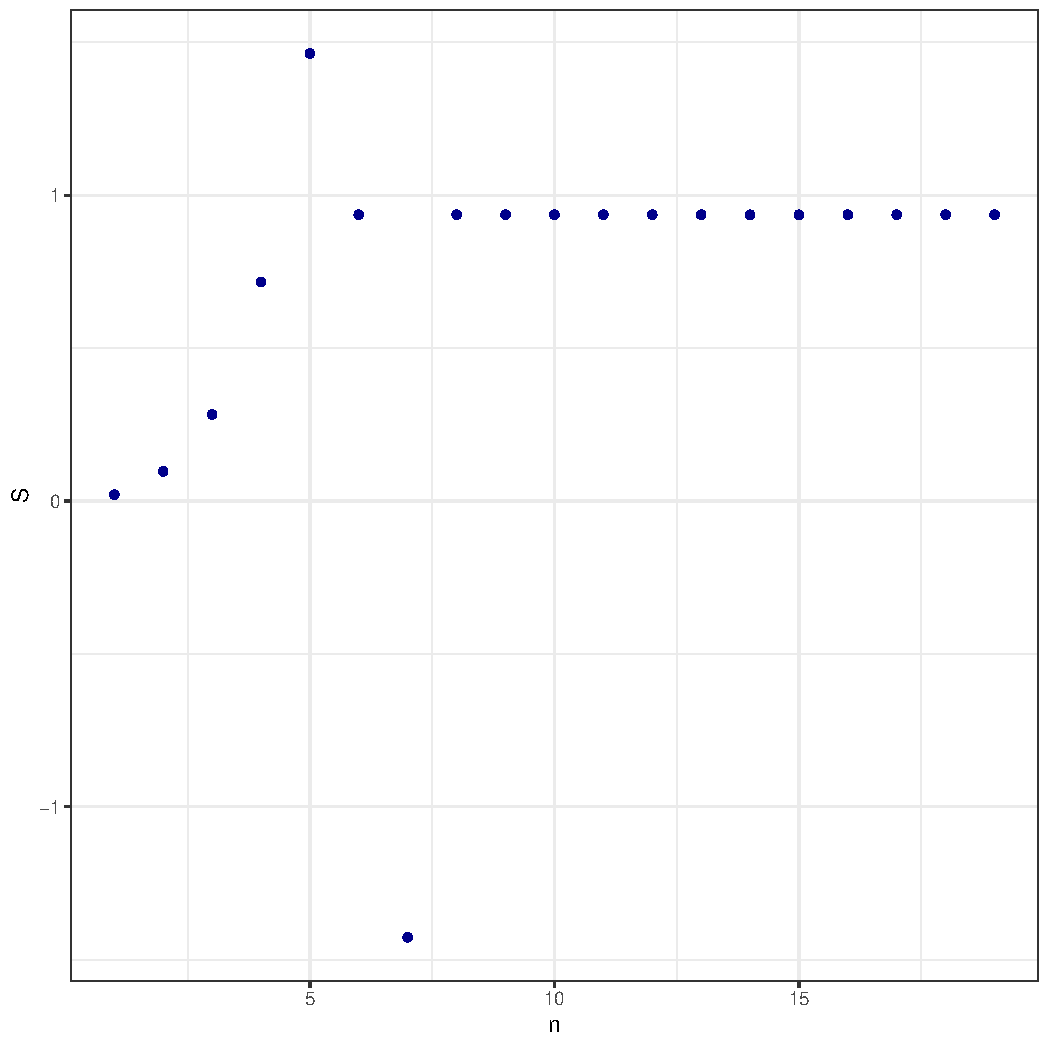
\includegraphics [width=3 in] {simpsons}} \caption{Simpsons method} \label{simpsons}
\end{figure}

Here we see that, with the exception of two outliers, the data approaches the value of S.

\section{Problem 3b}

Here we look to find the same S value as in equation 6. This time using the adaptive Simpson's method.

Again, the simulation was run with $\delta$ this time ranging from $10^{-15}$ to $1$, The results plotted the S values against $\delta$

\begin{figure}[h!]
\centerline{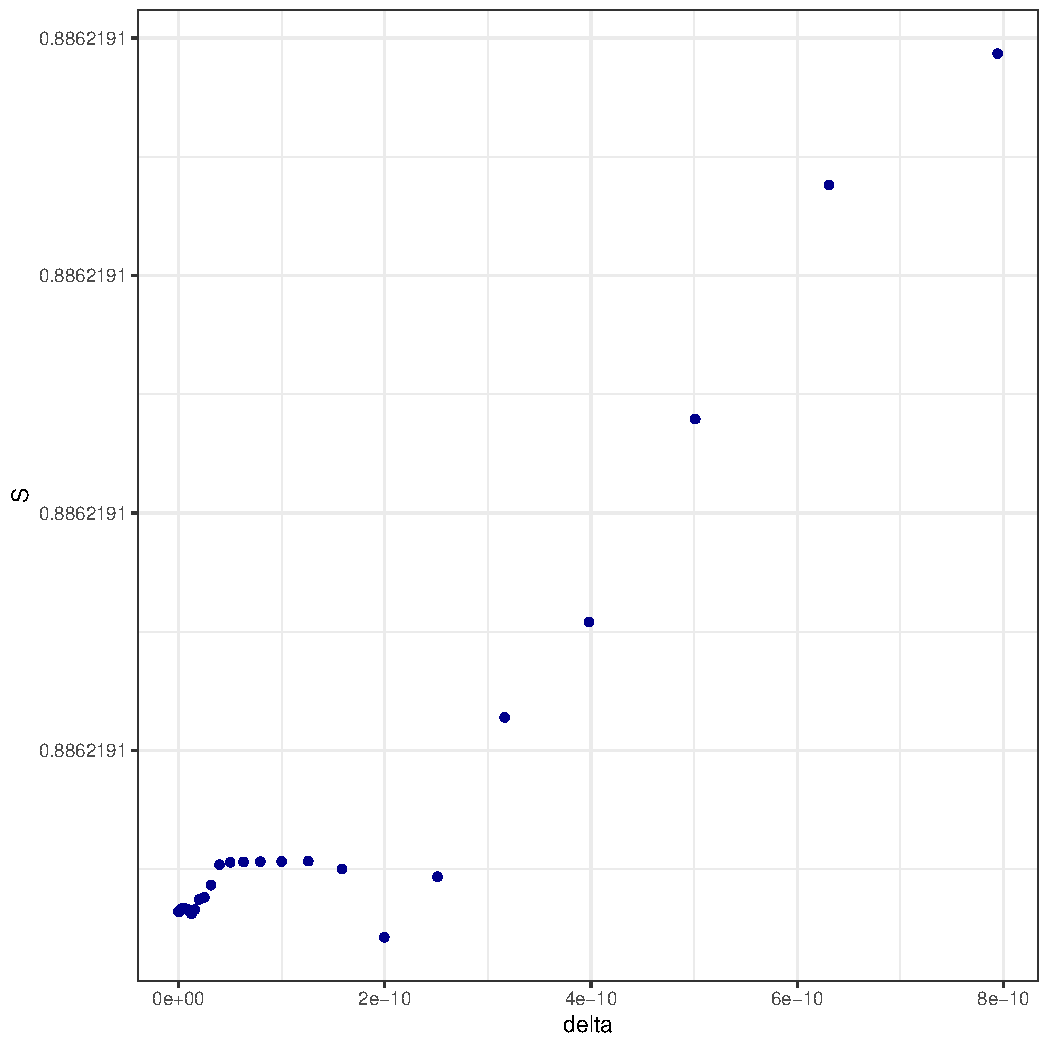
\includegraphics [width=3 in] {simpsons_adapt}} \caption{Simpsons method} \label{simpsons_adapt}
\end{figure}

Here is an interesting result. The plot almost looks like it's bouncing toward a value as a way of converging. It'ss converging to what is presumed to be $S$.

Make sure you include references to documents \cite{thecoursetext} you may have used.

\begin{thebibliography}{99}

\bibitem{thecoursetext} T. Pang, \emph{Introduction to Computational Physics}, Cambridge University Press (2006).

\end{thebibliography}

\end{document}